%==============================================================

\chapter{Results}\label{bds2}

Very small 100 Song Dataset plus 20 Cover Songs to evaluate and compare similarity metrics. Full similarity matrices. 
High performance/ throughput tests with full 12000 song testset to evaluate full load performance.\\

\section{Runtime}

\section{Cover song identification}

\textit{\textbf{Able to find "Rock you like a Hurricane" cover as top recommendation in over 11500 songs\\}}
\ \\
\textit{\textbf{counting the hits in the top 10 results of 80 requested songs on 164 song dataset covers80:\\}}
\begin{itemize}
	\item chroma: 16
	\item notes: 24
	\item chroma + notes: 24
	\item notes + rp: 22
	\item chroma + notes + rp: 28
	\item mfcc + notes + rp: 20
\end{itemize}
\textit{interesting sidenote: results of chroma only and notes only different! Nearly ever}

\section{Genre similarity}

\textbf{\textit{\underline{100 Song Testset, 10 genres:\\}}} 
\begin{figure}[htbp]
	\centering
	\framebox{\parbox{1\textwidth}{ 			
			\begin{subfigure}{.495\textwidth}
				\centering    
				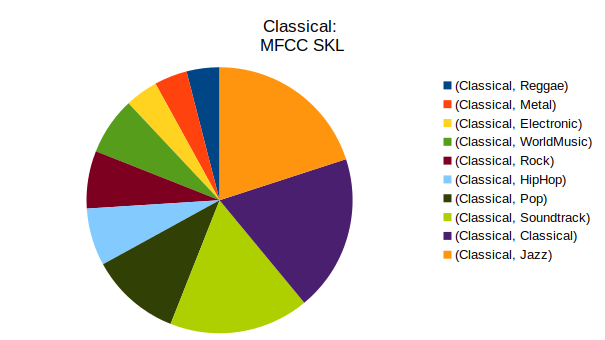
\includegraphics[scale=0.3]{Images/SparkFeat/Classical_MFCC_SKL.png}
				\caption{Classical MFCC SKL}
				\label{cms}
			\end{subfigure}		
			\begin{subfigure}{.495\textwidth}
				\centering     
				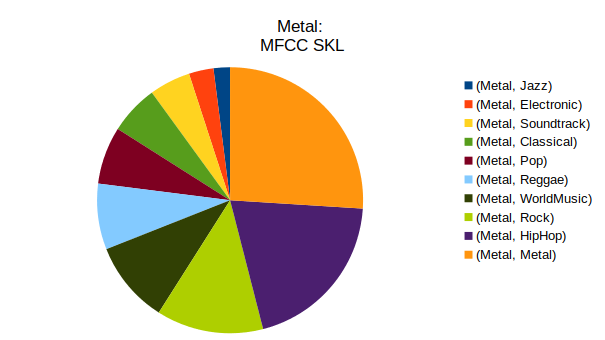
\includegraphics[scale=0.3]{Images/SparkFeat/Metal_MFCC_SKL.png}
				\caption{Metal MFCC SKL}
				\label{mms}
			\end{subfigure}%	
			
			\begin{subfigure}{.495\textwidth}
				\centering    
				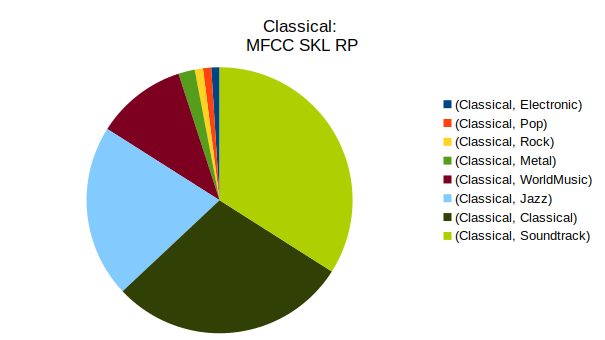
\includegraphics[scale=0.3]{Images/SparkFeat/Classical_MFCC_SKL_RP.png}
				\caption{Classical MFCC SKL RP}
				\label{cmsr}
			\end{subfigure}
			\begin{subfigure}{.495\textwidth}
				\centering     
				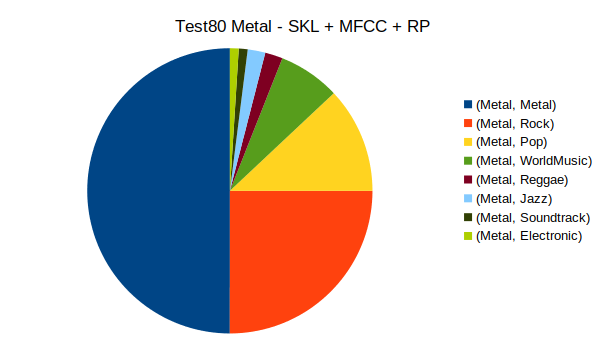
\includegraphics[scale=0.3]{Images/SparkFeat/Metal_MFCC_SKL_RP.png}
				\caption{Metal MFCC SKL RP}
				\label{mfsr}
			\end{subfigure}%		
	}}
	\caption{genre recall 100 songs}
	\label{fig:genrerec}
\end{figure}


\section{... and beyond genre boundaries}

\textit{\textbf{Rachmaninoff Prelude C\# minor full dataset Top 5 MFCC Euclidean\\}}
\\
\begin{itemize}
\item Songs/Klassik/Rachmaninoff-IdilBiret-Op3\_No2PreludeinC-SharpMinormp3
\item Jazz\&Klassik/100MeisterwerkederKlassik/Rachmaninov\_PianoConcertoNo2InCMinorOp18-1Moderato(Excerpt)mp3
\item Jazz\&Klassik/LangLang-Liszt/11\_LangLang\_PianoConcertoNo1inEflatmajorS124(LWH4)1Allegromaestosomp3
\item Jazz\&Klassik/PianoCollection/CD4-Brahms/03PianoSonataN°2inFsharpminorOp2-IIIScherzoallegrowav
\item Metal\&Rock/Compilations/RelapseSampler-RelapseSampler2015/SteveMoore-RelapseSampler2015-35Intro\&Creditsmp3
\item Jazz\&Klassik/LangLang-Liszt/12\_LangLang\_PianoConcertoNo1inEflatmajorS124(LWH4)2QuasiAdagio-Allegrettovivace-Allegroanimatomp3
\end{itemize}

\section{Improvements and outlook}

fma dataset\\
more state of the art similarity (blocked)\\
performance improvements\\

\section{Definition of similarity}
\textit{Rhythm, Timbre, Melodic, Genre and metadata, Genre specific features, combinations and variable model, Collaborative Filtering, Lyrics}

\textit{reduce hubness}

%\addtolength{\textheight}{-12cm}   % This command serves to balance the column lengths
% on the last page of the document manually. It shortens
% the textheight of the last page by a suitable amount.
% This command does not take effect until the next page
% so it should come on the page before the last. Make
% sure that you do not shorten the textheight too much.